\section{Bartłomiej Burczyk}
\label{sec:Bartlomiej}

\begin{enumerate}
    \item Number1
    \item Number2
    \item Number3
\end{enumerate}

\begin{itemize}
    \item Dot1
    \item Dot2
    \item Dot3
\end{itemize}


\begin{table}[h]
\centering
\begin{tabular}{||c c c c||} 
 \hline
 Crystal & Stone & Gas & Metal \\ 
 \hline\hline
 Diamond & Granit & Oxygen & Iron \\ 
 \hline
 Emerald & Marble & Nitrogen & Gold \\
 \hline
 Sapphire & Basalt & Hydrogen & Silver \\
 \hline
\end{tabular}
\label{tab:minerals}[]
\end{table}


\begin{figure}[htbp]
    \centering
    \caption{A dragon is a large magical legendary creature that appears in the folklore of multiple cultures worldwide. Beliefs about dragons vary considerably through regions, but dragons in Western cultures since the High Middle Ages have often been depicted as winged, horned, and capable of breathing fire.
    Dragons in eastern cultures are usually depicted as wingless, four-legged, serpentine creatures with above-average intelligence.}
    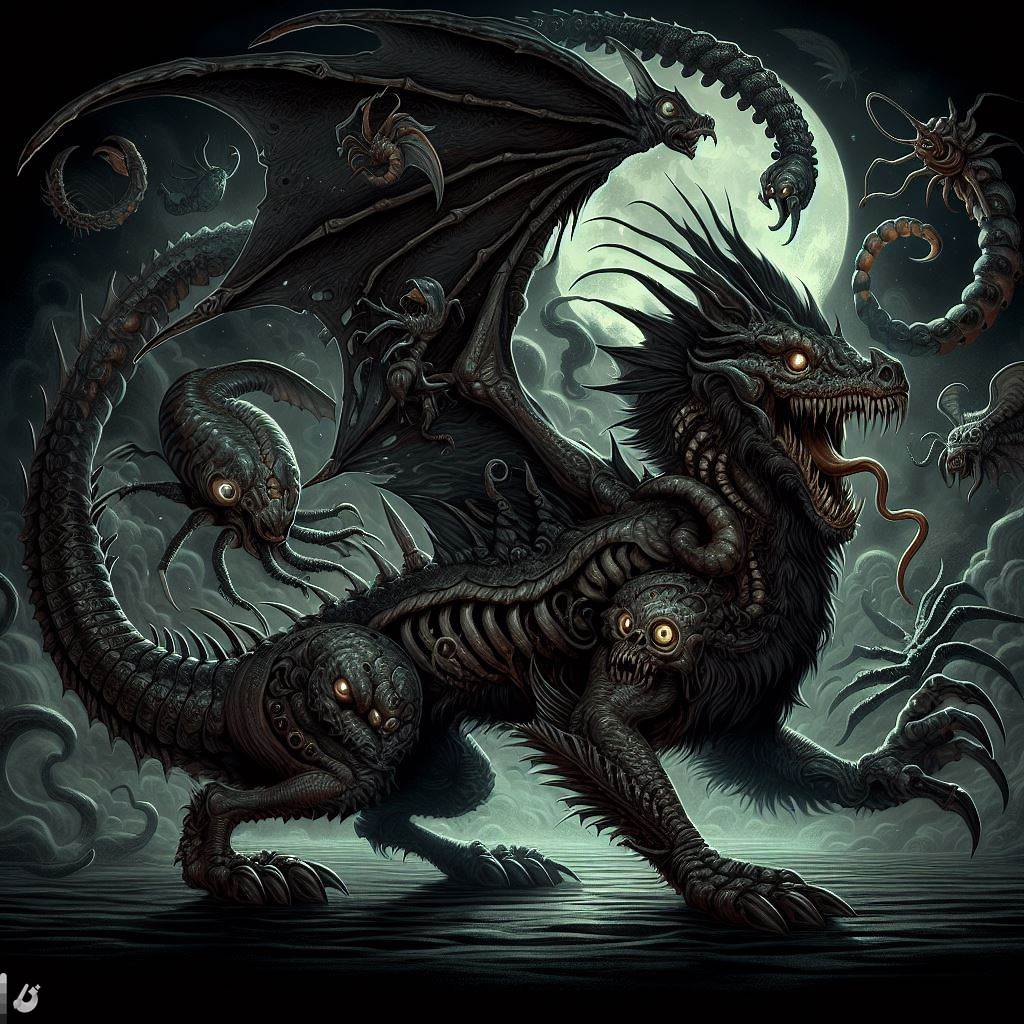
\includegraphics[width=0.5\textwidth]{pictures/dragon.jpg}

    \label{fig:dragon}
\end{figure}


\begin{figure}[ht]
    \[Area_{Circle}=\pi r^2\]
\end{figure}



